\documentclass[12pt]{article}
\usepackage[spanish]{babel}
\usepackage[utf8]{inputenc}     % Para que acepte acentos y ñ directamente
\usepackage[T1]{fontenc}        % Mejor manejo de caracteres acentuados
\usepackage{geometry}
\geometry{a4paper, margin=1in}
\usepackage{graphicx}
\usepackage{xcolor}
\usepackage{titlesec}
\usepackage{parskip}
\usepackage{multicol}
\usepackage{cite}
\usepackage{hyperref}           % Para hipervínculos en PDF
\hypersetup{
  colorlinks=true,
  linkcolor=blue,
  citecolor=blue,
  urlcolor=blue
}
\definecolor{highlight}{RGB}{255, 255, 0}

\titleformat{\section}{\normalfont\Large\bfseries}{\thesection}{1em}{}
\titleformat{\subsection}{\normalfont\large\bfseries}{\thesubsection}{1em}{}

\begin{document}

% Logos
\begin{minipage}{0.45\textwidth}
    
\includegraphics[width=0.4\textwidth]{inFiles/Figures/epnLogo.jpg}
\end{minipage}
\hfill
\begin{minipage}{0.45\textwidth}
    \raggedleft
    
\includegraphics[width=0.4\textwidth]{inFiles/Figures/FIS_logo.jpg}
\end{minipage}

\vspace{0.5cm}

% Títulos principales
\begin{center}
    \textbf{ESCUELA POLITÉCNICA NACIONAL}\\[0.2cm]
    \textbf{FACULTAD DE INGENIERÍA DE SISTEMAS}\\[0.2cm]
    \textbf{INGENIERÍA {\textbf{EN COMPUTACION}}}
\end{center}

\vspace{0.5cm}
\hrule
\vspace{0.5cm}

% Datos principales
\noindent\textbf{PERÍODO ACADÉMICO:} 2025-A\\[0.2cm]
\noindent\textbf{ASIGNATURA:} ICCD412 Métodos Numéricos \hfill \textbf{GRUPO:} GR2\\[0.2cm]
\noindent\textbf{TIPO DE INSTRUMENTO:} {Practica 2}\\[0.2cm]
\noindent\textbf{FECHA DE ENTREGA LÍMITE:}{04/05/2025}\\[0.2cm]
\noindent\textbf{ALUMNO:} {Lema Luis}

\vspace{0.5cm}
\hrule
\vspace{1cm}


% Secciones
\section*{TEMA}
{Tipos de errores}

\vspace{0.5cm}

\section*{OBJETIVOS}
\begin{itemize}
    \item {Analizar con profundidad los errores absoluto y relativo como herramientas clave para evaluar la precisión de los resultados numéricos,
     reconociendo su importancia en la toma de decisiones técnicas fundamentadas.}

     \item {Reflexionar sobre el impacto que tienen los errores de redondeo y truncamiento en los cálculos realizados por medios computacionales, 
     entendiendo cómo estas pequeñas variaciones pueden transformar el resultado final.}
\end{itemize}

\vspace{0.5cm}

\section*{MARCO TEÓRICO}
{En métodos numéricos, los errores son inevitables al aproximar valores. El error absoluto mide la diferencia 
directa entre el valor real y el aproximado,
 mientras que el error relativo lo expresa en términos de la magnitud del valor rea.} \cite{burden2015numerico}

  {Cuando trabajamos con constantes matemáticas como pi o e, a menudo usamos valores aproximados como 3.1416 o 2.718.
   Aunque estos valores facilitan los cálculos, siempre debemos considerar 
   cuán precisos son según el contexto del problema.} \cite{chapra2010canale}

  {También es importante entender los errores de redondeo, que ocurren al limitar los decimales en los cálculos,
   y los errores de truncamiento, que aparecen cuando cortamos una operación antes de terminarla (como una suma infinita).
    Ambos pueden afectar los resultados si no se controlan bien. } \cite{upv2023taylor}
 

\vspace{0.5cm}

\section*{DESARROLLO}
\begin{minipage}{0.95\textwidth}
    \raggedleft
    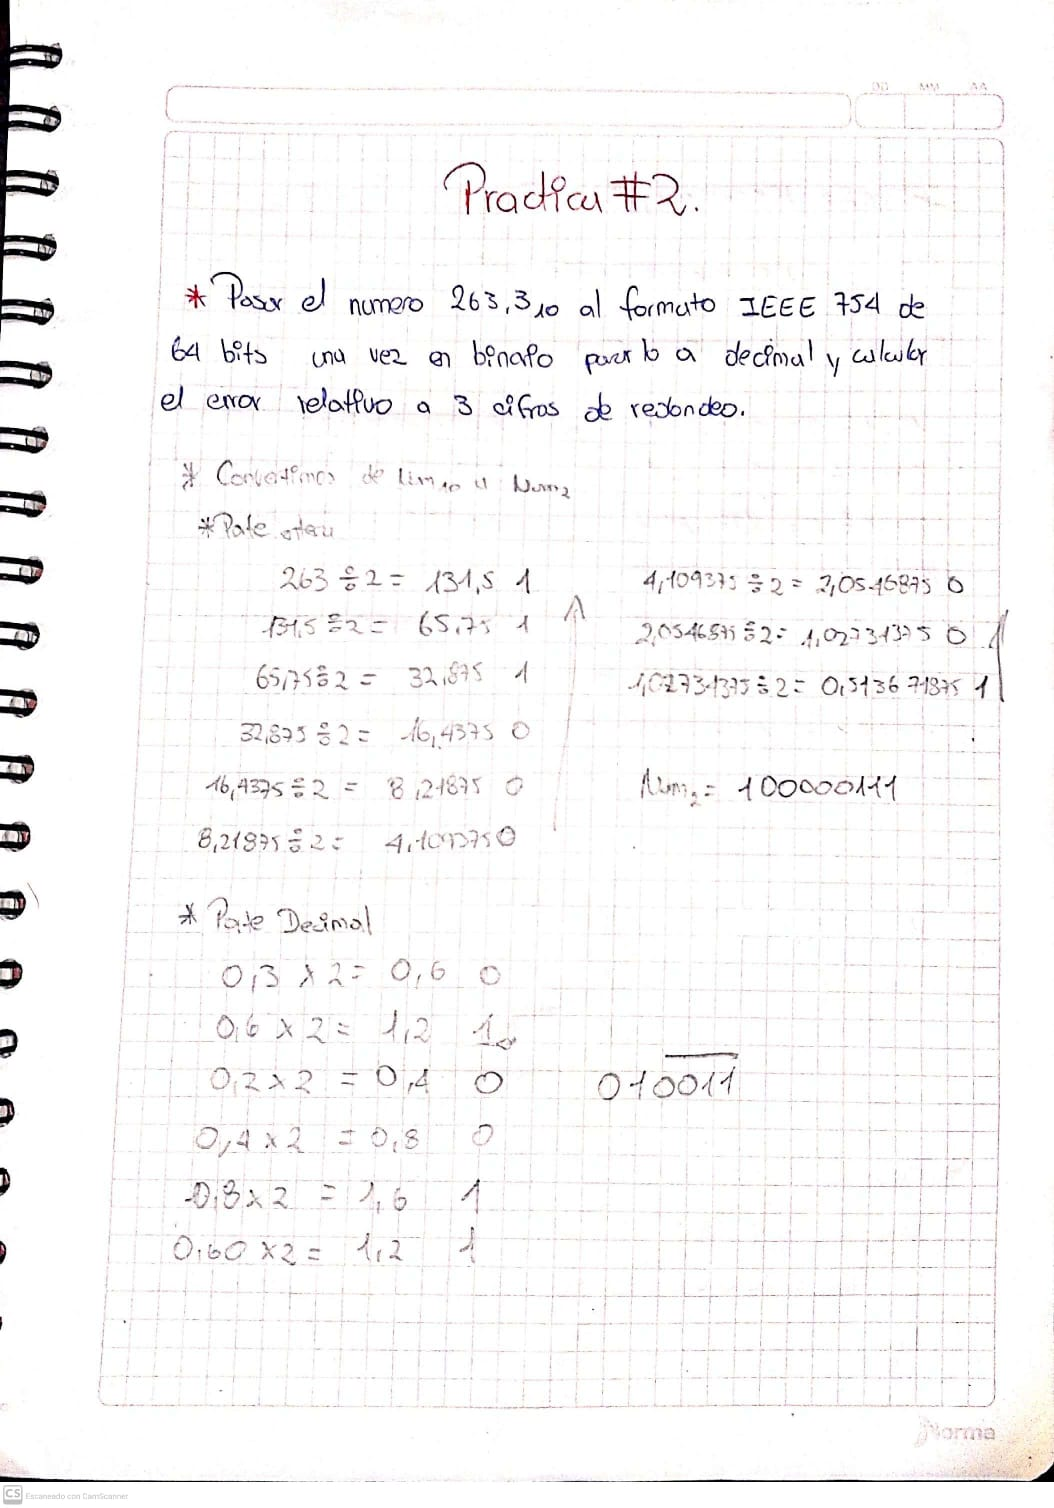
\includegraphics[width=0.95\textwidth]{inFiles/Figures/ej3.jpeg}
\end{minipage}

\vspace{0.5cm}

\begin{minipage}{0.95\textwidth}
    \raggedleft
    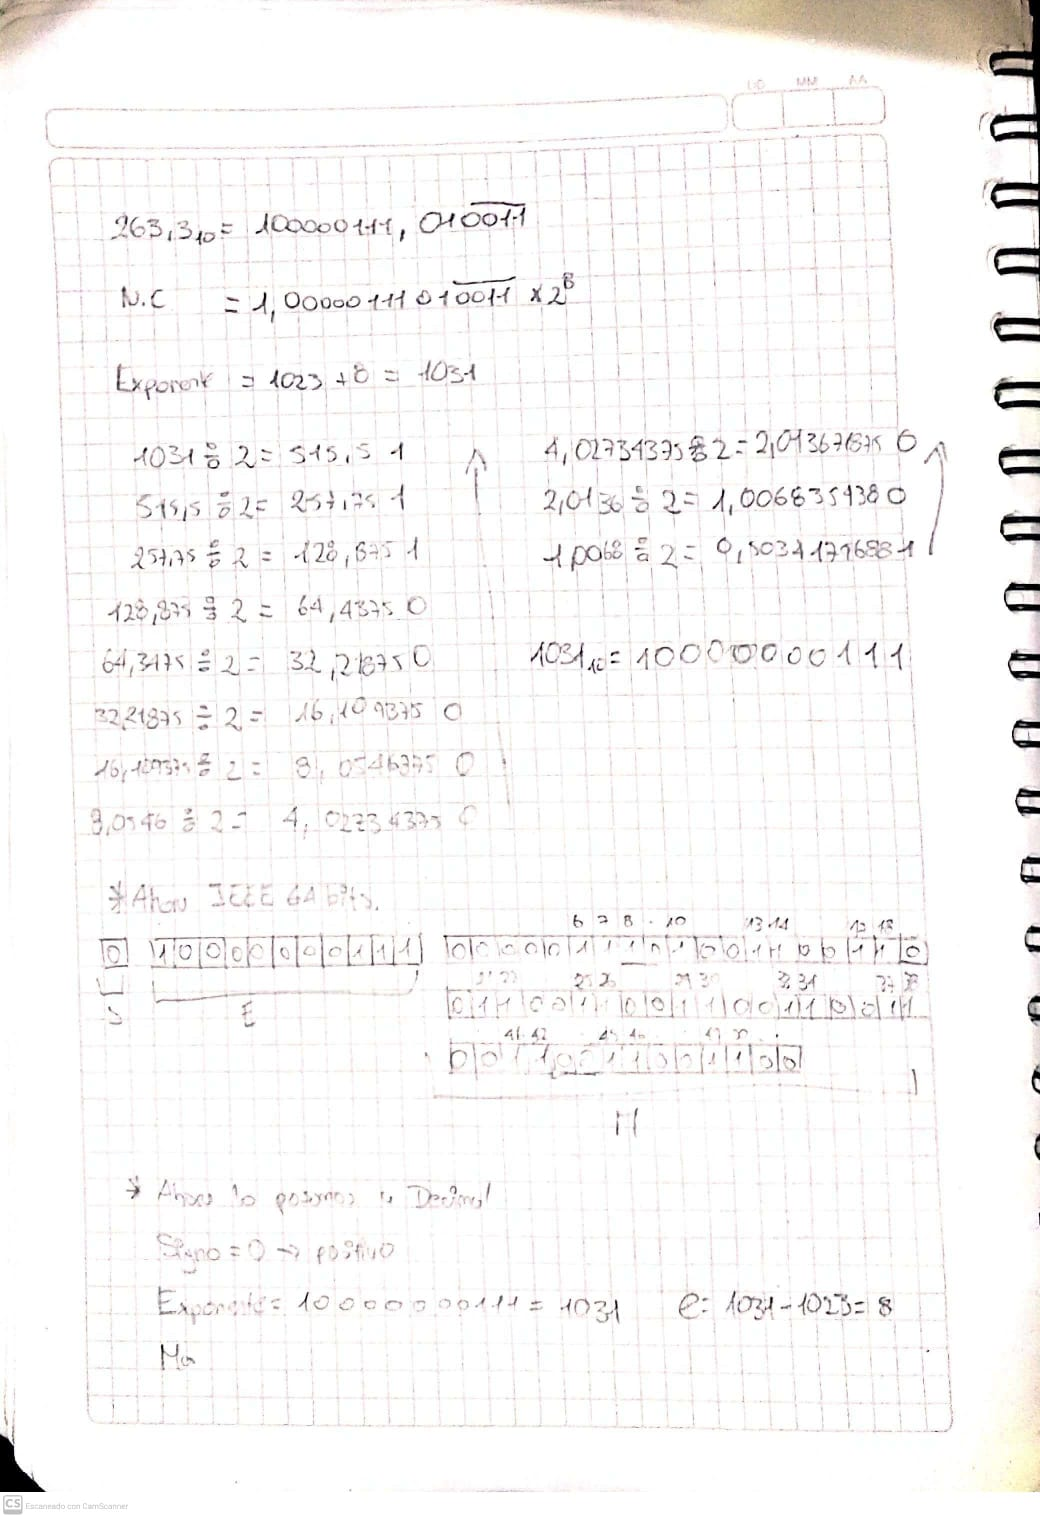
\includegraphics[width=0.95\textwidth]{inFiles/Figures/ej1.jpeg}
\end{minipage}

\vspace{0.5cm}

\begin{minipage}{0.95\textwidth}
    \raggedleft
    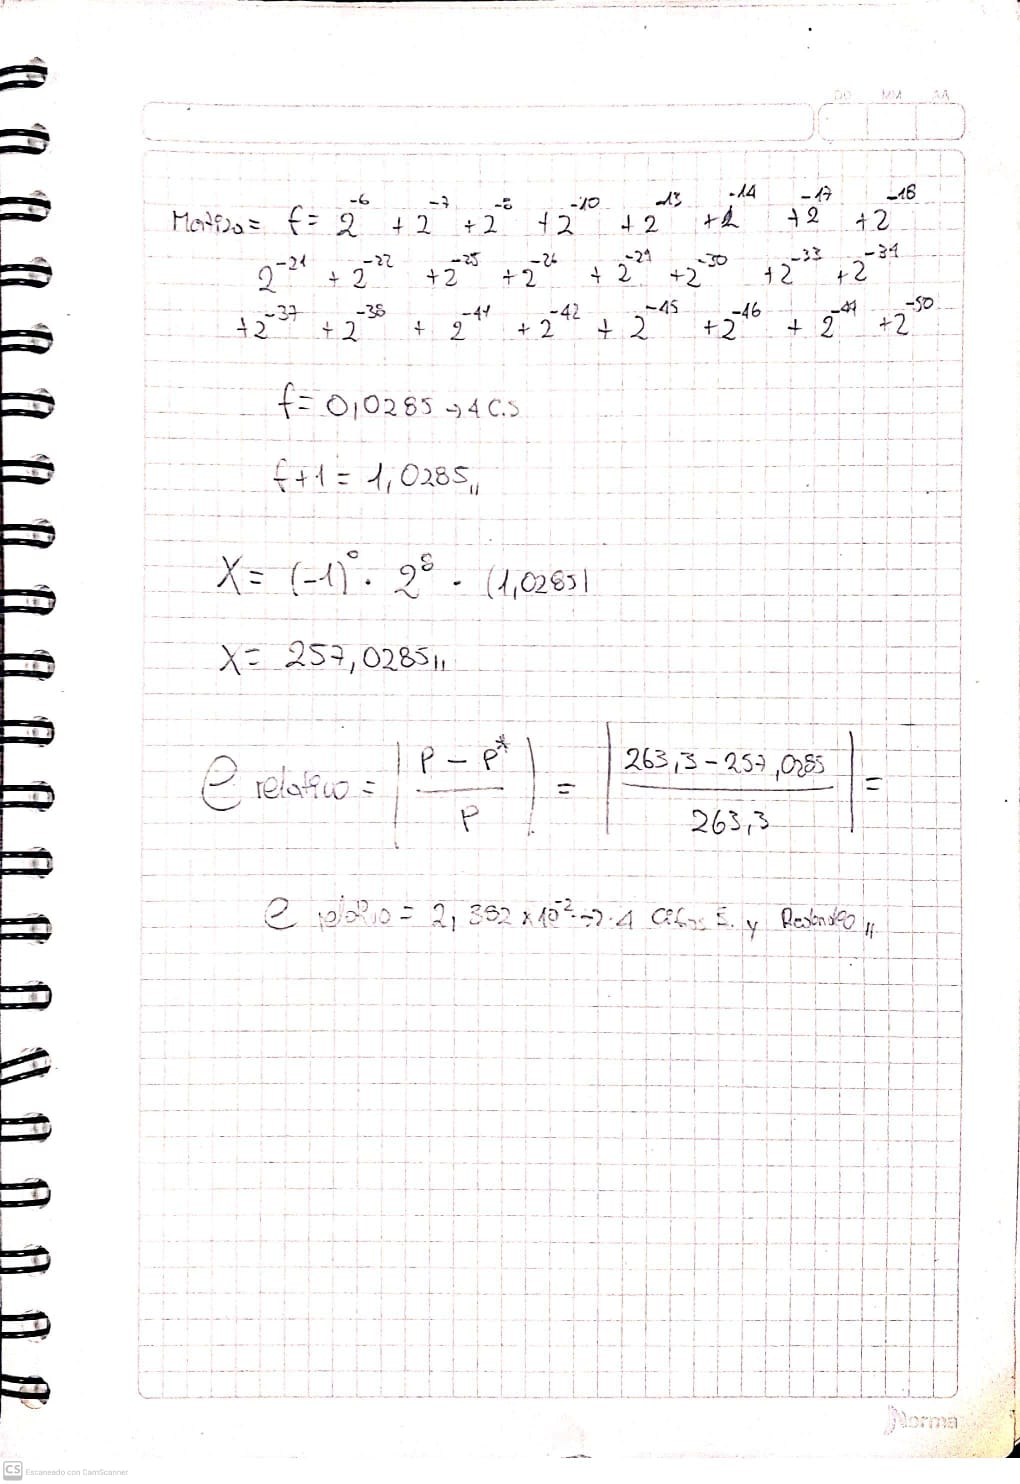
\includegraphics[width=0.95\textwidth]{inFiles/Figures/ej2.jpeg}
\end{minipage}

\vspace{3cm}


\section*{CONCLUSIONES}
\begin{itemize}
    \item {Medir los errores numéricos nos dio una visión más clara de qué tan cerca estamos del valor real 
    y qué tan confiables son nuestras aproximaciones.}
     \item {Las fórmulas no son lo único importante: saber cuándo y cómo usarlas hace toda la diferencia en el análisis numérico}
     \item {Esta práctica me ayudó a darme cuenta de que, en ingeniería, entender los errores no es un detalle técnico, sino una necesidad 
     para trabajar con responsabilidad.}
\end{itemize}


\vspace{0.5cm}

\section*{RECOMENDACIONES}
\begin{itemize}

     \item {Utilizar más decimales en los cálculos intermedios para evitar que el redondeo afecte el resultado final}
     \item {No confiar ciegamente en una aproximación solo por ser “conocida”; es mejor verificar su error relativo y ver si se ajusta a lo que se necesita}
     \
\end{itemize}


\vspace{0.5cm}


\renewcommand{\refname}{\MakeUppercase{REFERENCIAS}}
\bibliographystyle{IEEEtran}
\bibliography{inFiles/References/references.bib}
\end{document}
